\documentclass{beamer}
%
% Choose how your presentation looks.
%
% For more themes, color themes and font themes, see:
% http://deic.uab.es/~iblanes/beamer_gallery/index_by_theme.html
%
\mode<presentation>
{
  \usetheme{Hannover}      % or try Darmstadt, Madrid, Warsaw, ...
  \usecolortheme{beaver} % or try albatross, beaver, crane, ...
  \usefonttheme{serif}  % or try serif, structurebold, ...
  \setbeamertemplate{navigation symbols}{}
  \setbeamertemplate{caption}[numbered]
} 

\usepackage[english]{babel}
\usepackage[utf8x]{inputenc}
\usepackage{tikz}
\usetikzlibrary{mindmap,trees}
\usetikzlibrary{positioning}
\usepackage{verbatim}




%%%%%%%%%%%%%%%%%%%%%%%%%%%%%%%%%%%%%% DEFINICION FIGURAS TIKS:

\newcommand{\DrawAdjMat}{
	\node[nodo] (1) at (0,0) {$1$};
    \node[nodo] (2) [below = 0pt of 1] {2};
    \node[nodo] (3) [below = 0pt of 2] {3};
    \node[nodo] (4) [below = 0pt of 3] {4};
	\node[cell] (primero) [right = 0pt of 1] {T};
    \node[cell] (segundo) [right =0pt of primero] {T};
    \node[cell] (tercero) [right = 0pt of segundo] {F};
    \node[cell] (cuarto) [right = 0pt of tercero] {T};
    \node[nodo] (1c) [above = 0pt of primero] {1};
	\node[nodo] (2c) [above = 0pt of segundo] {2};
   	\node[nodo] (3c) [above = 0pt of tercero] {3};
    \node[nodo] (4c) [right = 0pt of 3c] {4};
   	\node[cell] (primero2) [right = 0pt of 2] {T};
    \node[cell] (segundo2) [right =0pt of primero2] {T};
    \node[cell] (tercero2) [right = 0pt of segundo2] {T};
    \node[cell] (cuarto2) [right = 0pt of tercero2] {F};
   	\node[cell] (primero3) [right = 0pt of 3] {F};
    \node[cell] (segundo3) [right =0pt of primero3] {T};
    \node[cell] (tercero3) [right = 0pt of segundo3] {T};
    \node[cell] (cuarto3) [right = 0pt of tercero3] {T};
	\node[cell] (primero4) [right = 0pt of 4] {T};
    \node[cell] (segundo4) [right =0pt of primero4] {F};
    \node[cell] (tercero4) [right = 0pt of segundo4] {T};
    \node[cell] (cuarto4) [right = 0pt of tercero4] {T};

	\begin{scope}[xshift = 3cm, yshift = -1mm,scale = 1.5]
    \foreach \pos/\nodo in {{(0,0)/1}, {(1,0)/2}, {(0,-1)/3}, {(1,-1)/4}}
        \node[vertex_adjMat] (\nodo) at \pos {\nodo};

    \foreach \start/\end in {1/2,1/4,4/3,2/3}
        \path[edge] (\start) -- (\end);
    \end{scope}
}

\newcommand{\DrawAdjList}{
    \node[nodo] (1) at (0,0) {$1$};
    \node[nodo] (2) [below = 0pt of 1] {2};
    \node[nodo] (3) [below = 0pt of 2] {3};
    \node[nodo] (4) [below = 0pt of 3] {4};
	\node[cell] (primero) [right = 0pt of 1] {2};
    \node[cell] (segundo) [right =0pt of primero] {4};
   	\node[cell] (primero2) [right = 0pt of 2] {1};
    \node[cell] (segundo2) [right =0pt of primero2] {3};
   	\node[cell] (primero3) [right = 0pt of 3] {2};
    \node[cell] (segundo3) [right =0pt of primero3] {4};
	\node[cell] (primero4) [right = 0pt of 4] {1};
    \node[cell] (segundo4) [right =0pt of primero4] {3};

	\begin{scope}[xshift = 3cm, yshift = -1mm,scale = 1.5]
    \foreach \pos/\nodo in {{(0,0)/1}, {(1,0)/2}, {(0,-1)/3}, {(1,-1)/4}}
        \node[vertex_adjMat] (\nodo) at \pos {\nodo};

    \foreach \start/\end in {1/2,1/4,4/3,2/3}
        \path[edge] (\start) -- (\end);
    \end{scope}
    }

\tikzset{every node/.append style={scale=0.75}}







%%%%%%%%%%%%%%%%%%%%%%%%%%%%%%%%%%%%%%%%%%%5












\title[GraphLib]{C++ GRAPH PROCESSING LIBRARY}
\author{Estructuras abstractas de datos y algoritmos}
\institute{Universidad de Costa Rica}
\date{10 Oct 2013}

\begin{document}

%Tikz styles definitions
\tikzstyle{vertex_adjMat}=[circle,fill=blue!25,minimum size=10pt,inner sep=2pt,font = \small]
\tikzstyle{cell} = [shape=rectangle,minimum size=15pt, inner sep=0pt,draw=black!50,fill=white, font=\scriptsize]
\tikzstyle{nodo} = [shape=rectangle,minimum size=15pt, inner sep=0pt,fill=white, font=\footnotesize]

\tikzstyle{vertex}=[circle,fill=blue!25,minimum size=10pt,inner sep=0pt,font = \tiny]
\tikzstyle{selected vertex} = [vertex, fill=red!24]
\tikzstyle{edge} = [draw,thick,-]
\tikzstyle{weight} = [font=\scriptsize]
\tikzstyle{selected edge} = [draw,line width=3pt,-,red!50]
\tikzstyle{ignored edge} = [draw,line width=3pt,-,black!20]
\tikzstyle{rojod edge} = [draw,line width=2pt,-,red!50]
\tikzstyle{rojog edge} = [draw,line width=4pt,-,red!70]
\tikzstyle{azul edge} = [draw,line width=4pt,-,blue!50]
\tikzstyle{arrow} = [fill=red!80, draw = black!20]
\pgfdeclarelayer{background}
\pgfsetlayers{background,main}



\begin{frame}
  \titlepage
\end{frame}

% Uncomment these lines for an automatically generated outline.
\begin{frame}{Outline}
  \tableofcontents
\end{frame}

\section{Introduction}

\begin{frame}{Introduction}
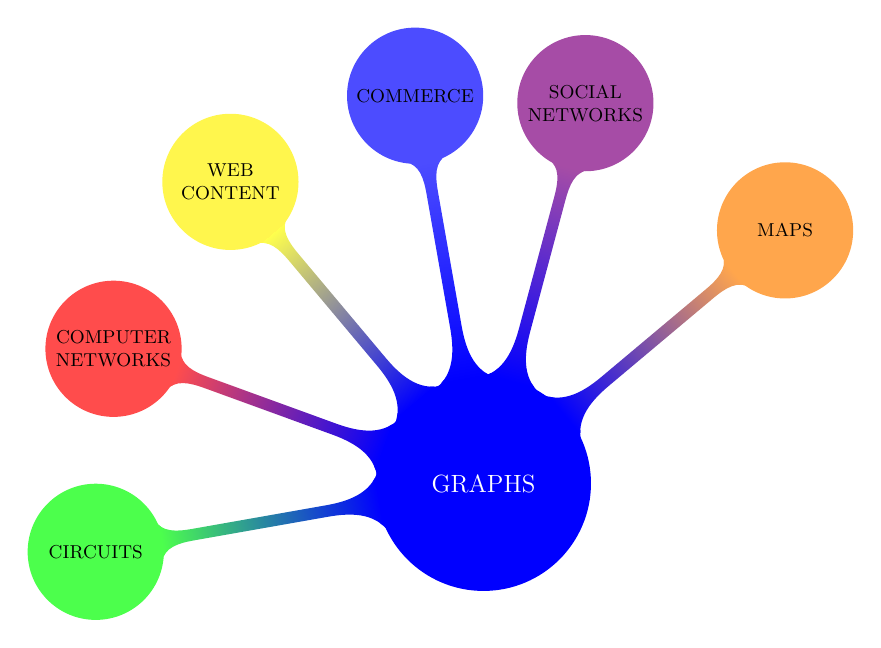
\begin{tikzpicture}
  \path[mindmap,concept color=blue,minimum size=1.5cm,text=white]
    node[concept] at (-10,50) {GRAPHS}
    [clockwise from=0]
    child[concept color=orange!70,grow=40,text=black] { node[concept] {MAPS} }
    child[concept color=yellow!70,grow=130,text=black] { node[concept] {WEB CONTENT} }
    child[concept color=green!70,grow=190,text=black] { node[concept] {CIRCUITS} }
    child[concept color=blue!70,grow=100,text=black] { node[concept] {COMMERCE} }
    child[concept color=red!70,grow=160,text=black] { node[concept] {COMPUTER NETWORKS} }
    child[concept color=violet!70,grow=75] { node[concept,text=black] {SOCIAL NETWORKS} };

\end{tikzpicture}
\end{frame}

\begin{frame}{Applications}
\begin{figure}
\centering
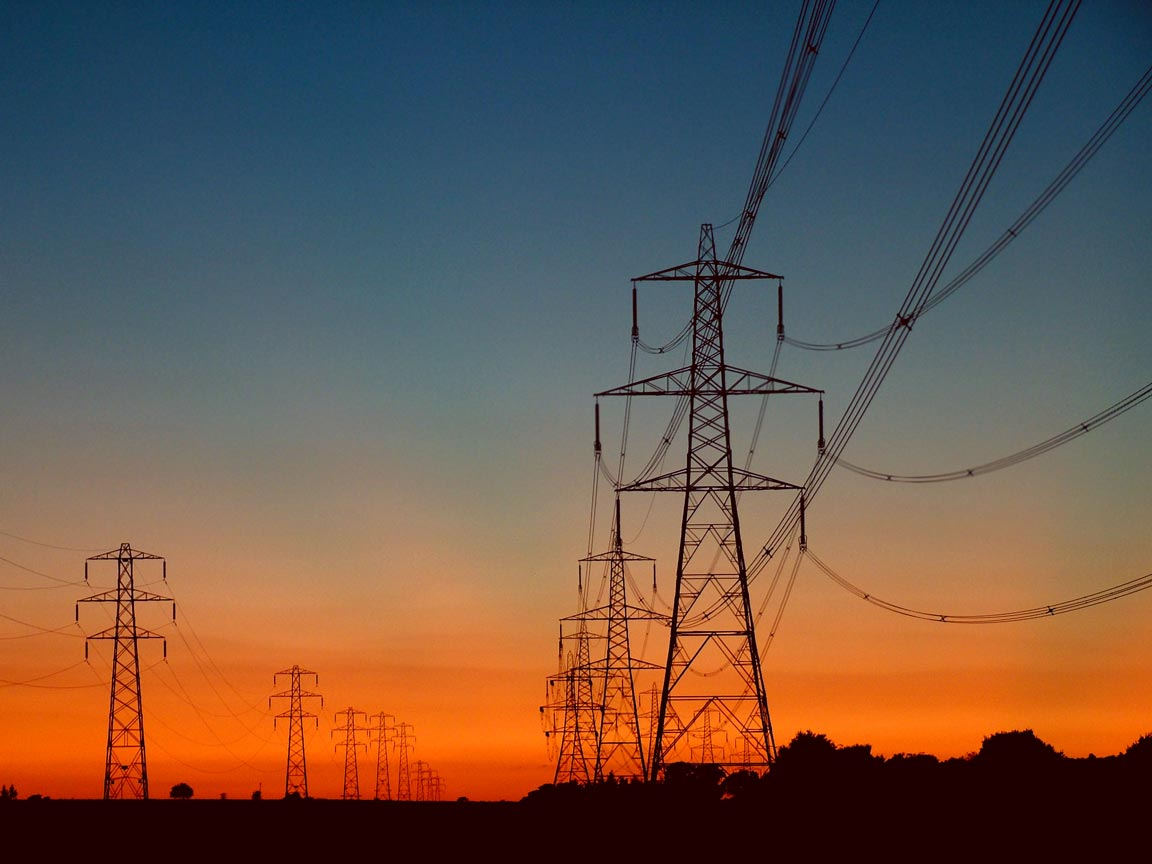
\includegraphics[width=.40\textwidth]{powerlines.jpg}
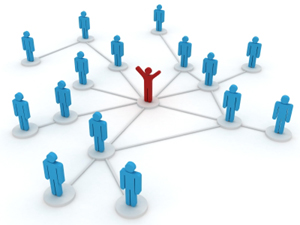
\includegraphics[width=.40\textwidth]{social-network.jpg}\\
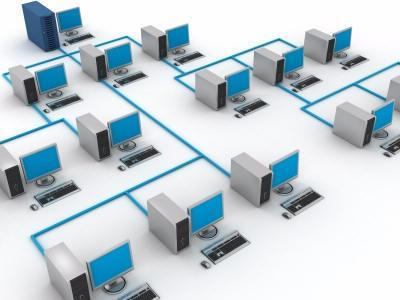
\includegraphics[width=.40\textwidth]{COMPNET.jpg}
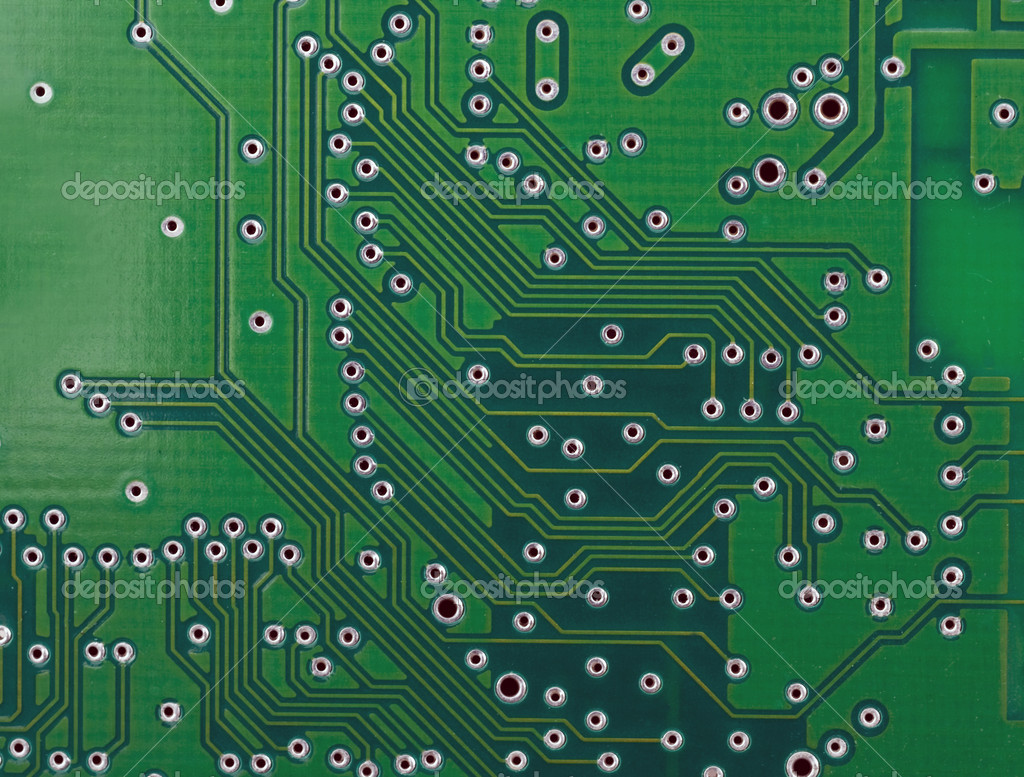
\includegraphics[width=.40\textwidth]{ic.jpg}\\
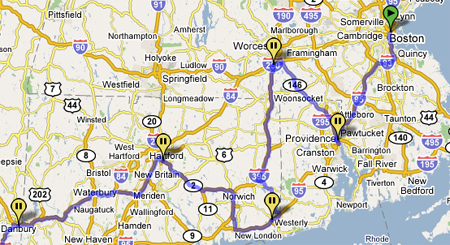
\includegraphics[width=.50\textwidth]{mapr.jpg}
\caption{Applications}
\end{figure}
\end{frame}

\begin{frame}{Definitions}


\begin{block}{Definition}
A graph is a set of vertices and a collection of edges that each connect a pair of vertices.
\end{block}


\begin{columns}[c]
\column{1.7in}
\begin{itemize}
  \item Vertex/Node
  \item Edge
  \item Path
  \item Cycle
  \item Connected - Unconnected Graph
  \item Length
  \item Tree, forest
\end{itemize}
\column{1.7in}
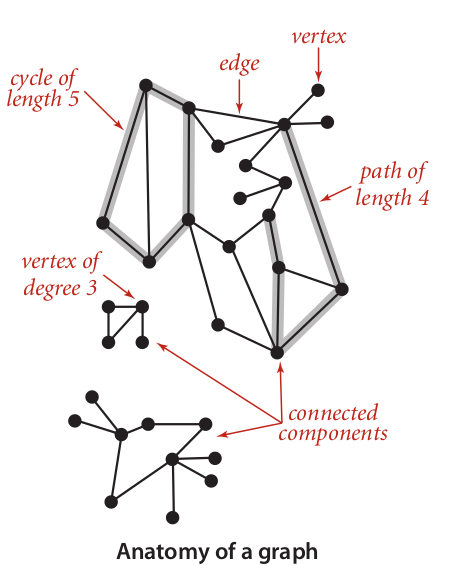
\includegraphics[width=1\textwidth]{Selection_024.png}
\end{columns}
\end{frame}

\begin{frame}{Data Structures}
\begin{columns}[c]
\column{1.7in}
\begin{figure}
	\begin{tikzpicture}
	\DrawAdjList	
	\end{tikzpicture}
    \caption{Adjacency List}
	\begin{tikzpicture}
	\DrawAdjMat	
	\end{tikzpicture}
    \caption{Adjacency Matrix}
\end{figure}
\column{1.7in}
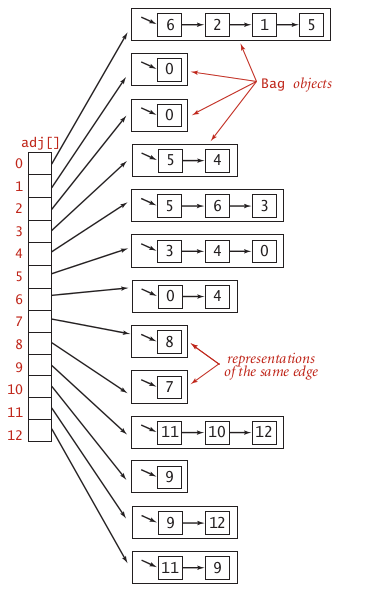
\includegraphics[width=1.1\textwidth]{adjl.png}
\end{columns}
\end{frame}

%%%%%%%%%%%%%%%%%%%%%%%%%%%%%%%%%%%%%%%%%%%%%5 ERNESTO
\section{Undirected Graphs}

\subsection{Aplications}
\begin{frame}{Definitions and applications}
%%%%
\end{frame}
\subsection{Algorithm 1}

\begin{frame}{ALgorithm 1}

\begin{itemize}
\item Use \texttt{tabular} for basic tables --- see Table~\ref{tab:widgets}, for example.
\item You can upload a figure (JPEG, PNG or PDF) using the files menu. 
\item To include it in your document, use the \texttt{includegraphics} command (see the comment below in the source code).
\end{itemize}

% Commands to include a figure:
%\begin{figure}
%\includegraphics[width=\textwidth]{your-figure's-file-name}
%\caption{\label{fig:your-figure}Caption goes here.}
%\end{figure}

\begin{table}
\centering
\begin{tabular}{l|r}
Item & Quantity \\\hline
Widgets & 42 \\
Gadgets & 13
\end{tabular}
\caption{\label{tab:widgets}An example table.}
\end{table}

\end{frame}

\subsection{Mathematics}

\begin{frame}{Readable Mathematics}

\end{frame}

\subsection{Algorithm 2}

\subsection{Algorithm 3}

%%%%%%%%%%%%%%%%%%%%%%%%%%%%%%%%%%%% HUGO

\section{Directed Graphs}
\begin{frame}
\end{frame}

%%%%%%%%%%%%%%%%%%%%%%%%%%%%%%%%%%%%%% 5 DIAPOSITIVAS DIEGO
\section{Minimum Spanning Trees}
\subsection{Applications}
\begin{frame}
%%%%%%%%%%%%%%%%%%%%%%%%%%
\end{frame}
\subsection{Definitions and data structures}
\begin{frame}
%%%%%%%%%%%%%%%%%%%%%%%%%%
\end{frame}
\subsection{Prim Algorithms}
\begin{frame}
%%%%%%%%%%%%%%%%%%%%%%%%%%
\end{frame}
\subsection{Kruskal Algorithm}
\begin{frame}
%%%%%%%%%%%%%%%%%%%%%%%%%%%%%%%%%%%%%%
\end{frame}

%%%%%%%%%%%%%%%%%%%%%%%%%%%%%%%%%%%% HUGO
\section{Shortest Paths}
\begin{frame}
\end{frame}
\end{document}
